\subsection*{d. Aumentar los precios de productos de la subcategoría Phones en un 8\%.}
Primero seleccionamos de la tabla \textit{products} los de la subcategoría \textit{Phones} y los guardamos en \textit{phones\_actuales}, que contiene los productos con su precio original y que serán los que se eliminen. Después, mediante una proyección sobre \textit{phones\_actuales}, conservamos las columnas \textit{productid}, \textit{category} y \textit{subcategory} y multiplicamos \textit{price} por 1.08, con lo que obtenemos \textit{phones\_actualizados}, que contiene los mismos productos pero con el precio aumentado en un 8\%. Para terminar, a la tabla \textit{products} le restamos \textit{phones\_actuales} y unimos \textit{phones\_actualizados}.

Expresión:
\begin{equation}
\begin{split}
& \left( products - \sigma_{subcategory = \text{'Phones'}}(products) \right) \\
& \quad \cup \; \pi_{productid,\, category,\, subcategory,\, price \cdot 1.08 \rightarrow price}\left(\sigma_{subcategory = \text{'Phones'}}(products)\right)
\end{split}
\end{equation}

Resultados obtenidos:

\begin{figure}[h!]
\centering
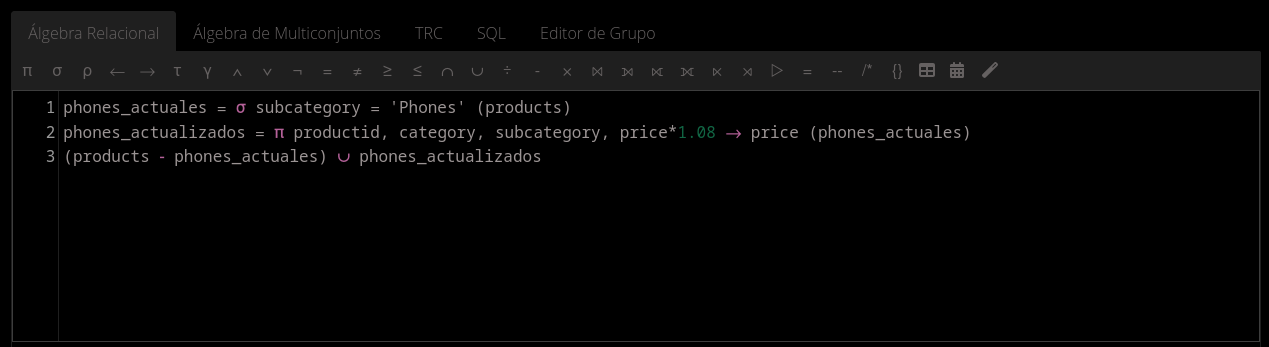
\includegraphics[width=0.8\textwidth]{imagenes/3d(1).png}
\caption{Consulta}
\end{figure}

\begin{figure}[h!]
\centering
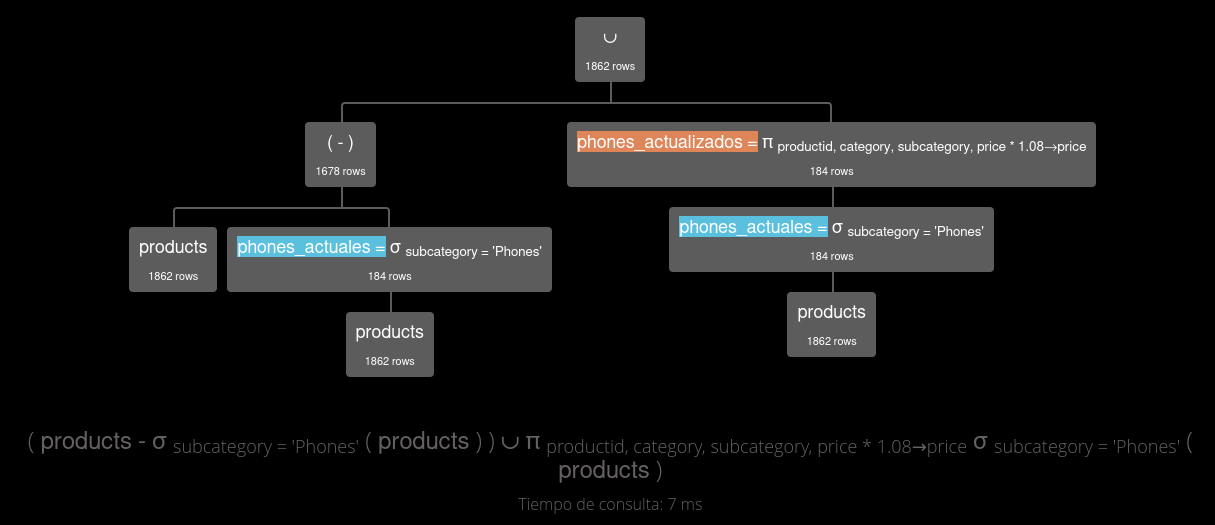
\includegraphics[width=0.8\textwidth]{imagenes/3d(2).png}
\caption{Árbol de consulta.}
\end{figure}

\begin{figure}[h!]
\centering
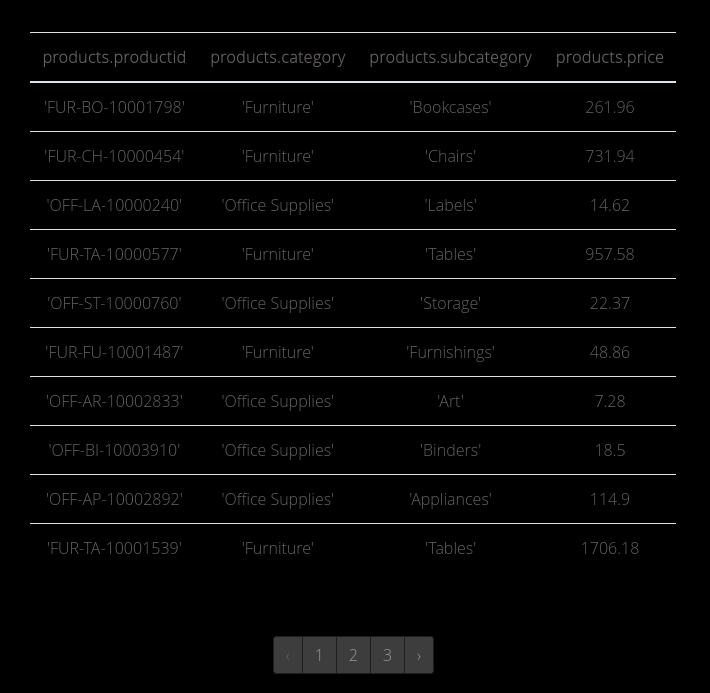
\includegraphics[width=0.6\textwidth]{imagenes/3d(3).png}
\caption{Resultado de consulta.}
\end{figure}